\chapter{Evaluation Methods}
In this chapter we will explain the metrics we use for evaluating our agents, then present our baseline agents.


\section{Evaluating Player Strength}
The goal of this work is to make test the viability of reinforcement learning for Schafkopf, which requires methods
of evaluation to test our agents playing strength.
We will outline three main strategies for this, that are reward earned overall, win percentage and expected value.

\subsection{Rewards Overall}
After each hand players are awarded a reward (See \ref{scoringphase}).
The total reward earned can be plotted on as Cumulative Sum for all players.
The Cumulative sum after N hands is calculated with:
\newline
\begin{center}
    Let r\textsubscript{i} be the reward earned in hand i then
    \begin{equation}
        \text{Reward after N Hands} = \sum_{i=1}^{N} r_{i}
    \end{equation}
\newline
    \begin{figure}[h]
    \centering
    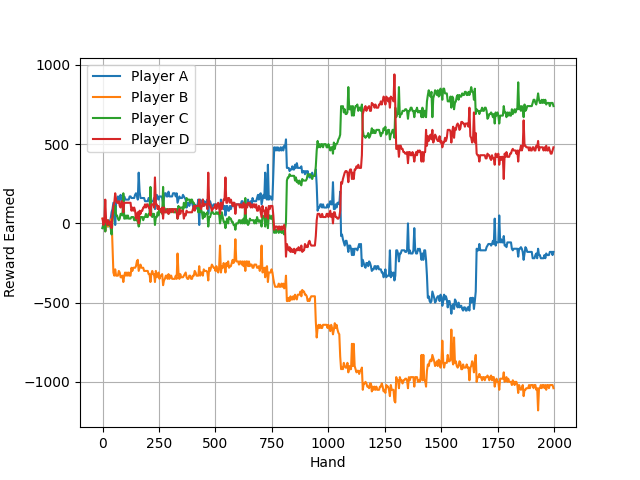
\includegraphics{expampleRewardEarned.png}
    \caption{Example of Rewards Earned for 4 Players after 2000 hands}
    \label{fig:exampleCumSum}
    \end{figure}
\end{center}
See Figure \ref{fig:exampleCumSum} for an example of this.\newline
This metric can be useful to get an initial idea of who is winning, but is susceptible to variance.\newline
Repeated trials often produce different results for players of equal strength.

\subsection{Win Percentage}
Firstly one can look at the overall win percentages across a sample of hands.
The win percentage can be calculated with the following formula.
\[\text{Win \%} = \frac{\# \text{ Hands Won}}{\# \text{ Hands Played}}\]
TODO example table
To achieve more detail of the agent's performance one we can further split the win percentage up into roles.
Overall there are seven roles in Schafkopf depending on the game mode, four offensive and three opposition:
\begin{itemize}
    \item Team
    \item Wenz
    \item Solo
    \item Team-Partner
    \item Team-Opposition
    \item Wenz-Opposition
    \item Solo-Opposition
\end{itemize}
For each of the seven roles we can then calculate separate win percentages with the formula above, replacing the
\textbf{Hands Won} and \textbf{Hands Played} with the respectively subset for each role.
\newline
This results for each player can then be shown in a table that allows for easy analysis of each role.
\newline
\begin{table}
\begin{tabular}{lrrrrrrr}
    \toprule
    Player & Team & Wenz & Solo & Team-Partner & Team-Opp & Wenz-Opp & Solo-
    Opp \\
    \midrule
    PlayerA & 0.506 & 0.917 & 0.864 & 0.527 & 0.505 & 0.167 & 0.226 \\
    PlayerB & 0.474 & 0.875 & 0.729 & 0.509 & 0.480 & 0.153 & 0.181 \\
    PlayerC & 0.527 & 1.000 & 0.829 & 0.518 & 0.511 & 0.194 & 0.214 \\
    PlayerD & 0.516 & 0.625 & 0.764 & 0.470 & 0.481 & 0.069 & 0.193 \\
    \bottomrule
\end{tabular}
\caption{Example of \textbf{winning percentage} for all seven roles for four players}
\label{winpercentageroles}
\end{table}
\newline
Win percentages are useful and would be sufficient if it were not for extra rewards \textit{Schneider} and
\textit{Schwarz}.
Two agents may have the same \textbf{winning percentage}, but one agent accumulates more rewards.

\subsection{Expected Value}
To address this we use \textbf{Expected Value(EV)}.
This concept is common in gambling games to express how much a certain bet or action, in our case hand, returns over
a large sample.
The formula used is the arithmetic mean:
\[ \text{EV} = \frac{1}{n} \sum_{i=1}^{n}a_{i} = \frac{a_{1} + a_{2} + ...+a_{n}}{n} \]
There are two hand metrics we can use for \textit{a\textsubscript{i}} of achieving this: \textbf{Points Scored} and
\textbf{Reward Earned}.

\subsection{Points Scored}
To calculate \textbf{EV\textsubscript{Points Scored}} of the hand sample we record the points scored and use the
above \textbf{EV} formula to calculate the metric.
\newline
\begin{table}[!h]
\centering
\begin{tabular}{cccc}
\toprule
Player A &  Player B &  Player C &  Player D\\
\midrule
32.48 & 33.71 & 27.49 & 26.32 \\
\bottomrule
\end{tabular}
\caption{EV\textsubscript{Points Scored} after 10000 games for four Players}
\label{tab:evscorestable}
\end{table}
\newline
In Table \ref{tab:evscorestable} we can see that Player A can expect to score 32.48 points per hand compared to only
the 26.32 of Player D.
In general we can say that Player A is the better player compared to Player B.
\newline
Although \textbf{EV\textsubscript{Points Scored}}certainly tells us something about playing strength, since Schafkopf
is after all a trick game, it also does not tell the whole story.
This metric scores greedy agents that only score for themselves higher than an agent that plays cooperative, even
though the cooperative agent might win more \textbf{Rewards} or even have a higher \textbf{Winning Percentage}.
\newline
It may certainly be useful but is not suitable to clearly evaluate an agent's playing strength.
Additionally one might also split up \textbf{EV\textsubscript{Points Scored}} further into the seven game role
categories, but this approach seems equally flawed.

\subsection{Rewards Earned}
To calculate \textbf{EV\textsubscript{Rewards Earned}} of the hand sample we record the rewards earned and use the
above \textbf{EV} formula to calculate the metric.
\newline
\begin{center}
\begin{table}[h!]
\begin{tabular}{cccc}
\toprule
Player A &  Player B &  Player C &  Player D\\
\midrule
2.32 &              2.92 &          -2.15 &          -3.08 \\
\bottomrule
\end{tabular}
\caption{Example of EV\textsubscript{Rewards Earned} after 10000 games for four Players}
\label{tab:EVrewardsOverall}
\end{table}
\end{center}
Table \ref{tab:EVrewardsOverall}] shows for example that Player A can expect +2.32 \textit{Reward} per hand, while
Player D can expect to lose -3.08 \textit{Reward} per hand.
To look closer at the areas that cause this we can also look again at the game roles.
\newline
\begin{center}
\begin{table}[h!]
\begin{tabular}{lrrrrrrr}
\toprule
Player &  Team &    Wenz &   Solo &  Team-Partner &  Sauspiel-Opp &  Wenz-Opp &  Solo-Opp \\
\midrule
Player A &  4.93 &   39.58 &  84.39 &          2.39 &         -0.48 &     87.89 &     -2.83 \\
Player B &  4.27 &  131.48 &  79.03 &          6.08 &          1.61 &    -47.73 &     -6.85 \\
Player C &  2.03 &  -21.07 &  13.42 &         -2.21 &         -5.46 &    -34.35 &    -80.14 \\
Player D & -2.88 &  -23.68 &   6.31 &          1.51 &         -6.18 &   -235.00 &    -98.13 \\
\bottomrule
\end{tabular}
    \caption{Example of EV\textsubscript{Rewards Earned} by game role after 10000 games for four Players}
\label{tab:EVrewardsGamemode}
\end{table}
\end{center}
\textbf{EV\textsubscript{Rewards Earned}} overcomes the previous pitfall.
It more accurately shows when agents extract value from additional rewards earned, which was not possible by simply
looking at the \textbf{Winning Percentages}, or while also taking into account the advantage of cooperative play.
\newline
\textbf{EV\textsubscript{Rewards Earned}} will be the main tool when considering playing strength.


\section{Hand Seeding \& Fairness}
To evaluate player strength we introduced seeding as it is a way to reduce variance in the game.
This concept is for example used in competitive Bridge and Scrabble[REF] as a means for fairness, since card games
often have a high degree of variance.
This variance and the low number of games played at competitive would otherwise make any competition part lottery.
\newline
For Schafkopf there are three features that define a hand:
\begin{description}
    \item [Hand distribution] The way the cards are distributed to the four seats at the table.
    \item [Relative Hand Position] Hand A sits to the right of Hand B and so on.
    \item [Initial Lead] Who starts the hand determines not just the play but also the Bidding.
\end{description}
Although fairly obvious, they act as a minimal and sufficient way of describing the initial state of a game.
In order to control for these, a seeding mechanism was introduced that can be called when initialising the game
environment.
This alone however is not enough to reduce the variance between four players, as it only allows to control the
seeding between two tables of players.
\newline
If we imagine a tournament in which the 12 hands (or three rounds) are played at Table A and Table B, so that A and B
receive the same hands, in order to find the best player among both tables.
It might happen that the majority of hands are favourable for Seat 1, and the player in that seat wins by a big margin.
The same or similar would happen on Table B and no one is the wiser to who is the strongest player.
\newline
To get around this, we introduced "Fair tournaments" that play each seed four times, each player gets to play the hand
from every seat once.
[IMAGE of rotation]
[CODE Fair tournament]
This way, player strength can be evaluated to a good degree, since good cards cancel out and marginal
advantages in playing strength are rewarded.
Agent 1 might score with accurate play for the same seed more reward the Agent 2 by receiving an extra reward for
Schneider.
\newline
As a last point, it should be said that there is still some variance due to the players.
Firstly most players (and also agents used here) do not play completely deterministic, thus sometimes they make
incorrect decision, and this being an imperfect information game, two identical seeds will not produce the same game.
\newline
On the other hand, the order the players sit at the table may also have some effect.
Player A,B,C and D, all of differing strength, can have [FORMULA]4! seating arrangements that would each have to be
played four times.
\[\text{Hands per Seed} = 4! * 4 = 96\]
96 hands per seed would be more fair, but seems in the scope of this work unnecessary and due to the above
potentially still not sufficient.

In order to test our networks we designed baseline agents to play against, to measure playing strength.
The agents all use same \textit{makebid()} method to establish an even playing field, on which we can compare pure
playing strength.
Each agent's strategy will be briefly explained and statistics from a fair tournament, which is played between four
instances of the respective player,will be given to get an idea of their perfomance.
\newline
See Table \ref{tab:baselinevs} for an inbetween comparison of three baseline agents, each playing 10000 hands
against each other.
\begin{table}[!h]
    \centering
    \begin{tabular}{lccc}
        \toprule
        Player    & Random & Greedy & Heuristic \\
        \midrule
        Random    & -      & -4.55  & -5.48     \\
        Greedy    & 4.55   & -      & -1.35     \\
        Heuristic & 5.48   & 1.35   & -         \\
        \bottomrule
    \end{tabular}
    \caption{Baseline agent tournament that shows the order of strenght in accending order: Random, Greedy, Heuristic}
    \label{tab:baselinevs}
\end{table}


\section{Static Bidding}
Table \ref{tab:distributionBidding} shows the distribution of contracts.
We can see that the majority of hands are Team contracts, whilst the remaining 15\% of games are envenly distributed
over the remaining Solo contracts.\\
The bidding heuristic used here is by no means expert play but overall reasonable for what we are trying to achieve.
Human players are likely to play a somewhat higher percentage of Solo games, although that frequency is heavily
affected of one's one playing strength, and ideally varied according to one's opponents abilities.
To find a balance between win rate and winning frequency is major part in contract card games such as Bridge and
Schafkopf.
\begin{table}[!h]
    \centering
    \begin{tabular}{lc}
        \toprule
        Contract    & Distribution \\
        \midrule
        Team        & 85,3         \\
        Wenz        & 6,6          \\
        Colour-Solo & 8,1          \\
        No Game     & 0,0          \\
        \bottomrule
    \end{tabular}
    \caption{Distribution of contracts}
    \label{tab:distributionBidding}
\end{table}


\section{Baseline Agents}
The following table shows the baseline comparison between the three baseline agents, each playing 10000 hands against
one another.

\subsection{Random Agent}
The Random agent plays like the name suggests a random valid card.
It makes no use of the passed games state, has no understanding of team composition and performs expectantly bad.
This strategy is terrible for all contracts, although some hands can still be played near optimal, due to holding good
cards, having competent teammates, or having little choice.
\begin{table}[!h]
    \centering
    \begin{tabular}{ccccccc}
        \toprule
        Team  & Wenz  & Solo  & Team-Partner & Sauspiel-Opp & Wenz-Opp & Solo-Opp \\
        \midrule
        0.616 & 0.539 & 0.843 & 0.616        & 0.384        & 0.461    & 0.157    \\
        \bottomrule
    \end{tabular}
    \caption{Average win rates of Random agent against itself over 10000 hands}
    \label{tab:winratesRan}
\end{table}

\subsection{Greedy Agent}
The Greedy agent will always try to win every trick possible.
It understands trumps, tricking, point values, but has no understanding of team composition.
When he has the lead it chooses to play the highest rank that is not trump, or the highest trump if it only holds trump.
When not in the lead it will test if it can beat the cards in the current trick, even if one of his partner currently
is the trick winner.
If it holds more than one winning card it will choose the card with the highest point value.
Vice Versa if it holds no winning card it will choose the lowest point value card, if possible not trump, even if
that means playing an Ace.\\
In summary,Greedy agent values winning tricks and not giving up trump if possible.
This strategy can certainly be viable for Solo contracts where itself is the bid winner, but will fail when it is
part of the opposition, because trumps are sparse and over-tricking teammates is major error.
For team contracts it [LOOK at stats, might be ok for]
\begin{table}[!h]
    \centering
    \begin{tabular}{ccccccc}
        \toprule
        Team  & Wenz  & Solo  & Team-Partner & Sauspiel-Opp & Wenz-Opp & Solo-Opp \\
        \midrule
        0.604 & 0.646 & 0.757 & 0.604        & 0.396        & 0.354    & 0.243    \\
        \bottomrule
    \end{tabular}
    \caption{Average win rates of Greedy agent against itself over 10000 hands}
    \label{tab:winratesGre}
\end{table}

\subsection{Heuristic Agent}
The Heuristic agent is a lot more nuanced than the above agents.
It employs a separate strategy for each of seven game positions and uses the game state to infer the team composition
,if possible, and uses the strategies from \ref{basicstrategy} to some extent.\\
Furthermore it understands everything Greedy agent knows, about points, trump and tricking.
Its limitations are its use of the trick history, which is only used when it plays in the offensive or team partner
role to infer how many trumps are still with the others, but misses strategies, such as leading a suit where a
teammate is known to be, or similar.
The decision process is mostly deterministic, but there are situations where two cards are equally playable and one is
randomly chosen.\\
Heuristic agent is certainly a decent opponent that follows good practice play a novice might bring to the table.
\begin{table}[!h]
    \centering
    \begin{tabular}{ccccccc}
        \toprule
        Team  & Wenz  & Solo  & Team-Partner & Sauspiel-Opp & Wenz-Opp & Solo-Opp \\
        \midrule
        0.485 & 0.588 & 0.695 & 0.485        & 0.515        & 0.412    & 0.305    \\
        \bottomrule
    \end{tabular}
    \caption{Average win rates of Heuristic agent against itself over 10000 hands}
    \label{tab:win ratesHeu}
\end{table}